\chapter{Background and Related Work}
\label{chptr:concepts}

Introducing redundancy to safety-critical systems is a popular approach to ensure that faults inside the system do not lead to failures that effect the system's environment~\cite{BarryFaultToleranceAnalysis}.
Redundancy can be achieved in multiple ways, some of which being adding additional resources (hardware redundancy), adding additional information or messages (information redundancy), or performing the same operation multiple times (time redundancy).
Although being one of the most often used redundancy techniques, the addition of hardware components, called replicas for redundant computation, leads to multiple results which need to be consolidated to an unique system result.
Thus, the replicas need to communicate with each other and synchronize their results in order to act like a single unit in their environment.
A promising approach to cope with the communication overhead is \gls*{DDS}, a \gls*{DCPS} system, since it allows reliable and real-time communication~\cite{omgDDSspec}.
However, while hardware redundancy enhances a system's fault-tolerance, it also increases its costs and complexity.

In this chapter, various redundancy techniques, as well as important terms and criteria for evaluating redundant systems, are described.
Further, different redundancy concepts are weighted against each other with regards to reliability, safety, and performance.
Afterwards, standards for building and designing safe and fault-tolerant systems are given and related works, that sucessfully applied \gls*{DCPS}-middleware in the railway context, are shown.
At first, however, an overview about the \abr{ETCS}, as well as the \gls*{DDS} standard and its concepts, is exposed.

\section{\glsentryfull{ETCS}}
In order to facilitate interoperability between national railway systems throughout Europe, the signalling and speed control system has been standartized by the European Union under the term \abr{ERTMS}.
\abr{ETCS} defines the signalling and train control component of \abr{ERTMS}~\cite{ETCS26}.
As such, it is responsible for monitoring a train's speed, calculating the permissible speed restrictions, and coordinating the collaboration between track-side components, such as \abr{ETCS} eurobalises, and on-board systems.
Any train requires a permission in form of a \abr{MA} to drive from its location to another point on track.
Besides encoding a train's permission to move, a \abr{MA} also encodes information about other trains on the track, as well as track information such as slopes and speed limitation.
Any \abr{MA} is supplied by an external entity, called \abr{RBC}, via track-side components or via radio frequencies, and monitored by an on-train system.
The track-side components, as well as the on-board system, are standardized according to three different \abr{ETCS} levels.

\paragraph{\abr{ETCS} level one}
\abr{ETCS} level one has been designed to build upon existing signalling systems.
\abrpl{MA} as well as route data and the maximum allowed speed are transmitted through fix positioned eurobalises.
Parallel to that, a breaking curve and the train's position are permanently calculated.

\paragraph{\abr{ETCS} level two}
For \abr{ETCS} level two, signalling and \abr{MA} data is transmitted via mobile communication channels from the \abr{RBC} and displayed to the driver.
The \abr{RBC} is a central unit that constantly collects and supervises train movements and track information.
Although each train calculates its own position, it can come to inaccuracies, due to for example faulty sensor calibration.
Therefore, track-side balises are applied, whose exact positions are provisioned before the train's journey during a linking phase.
Thus, a train's actual position can be aligned when it encounters a linked balise.

\paragraph{\abr{ETCS} level three}
Finally, in \abr{ETCS} level three, any track-side component is abolished and the entire communication takes place via radio signals.
This \abr{ETCS} level is not fully standardized yet.

\section{\glsentryfull{DDS}}

\begin{figure}[!hb]
	\centering
	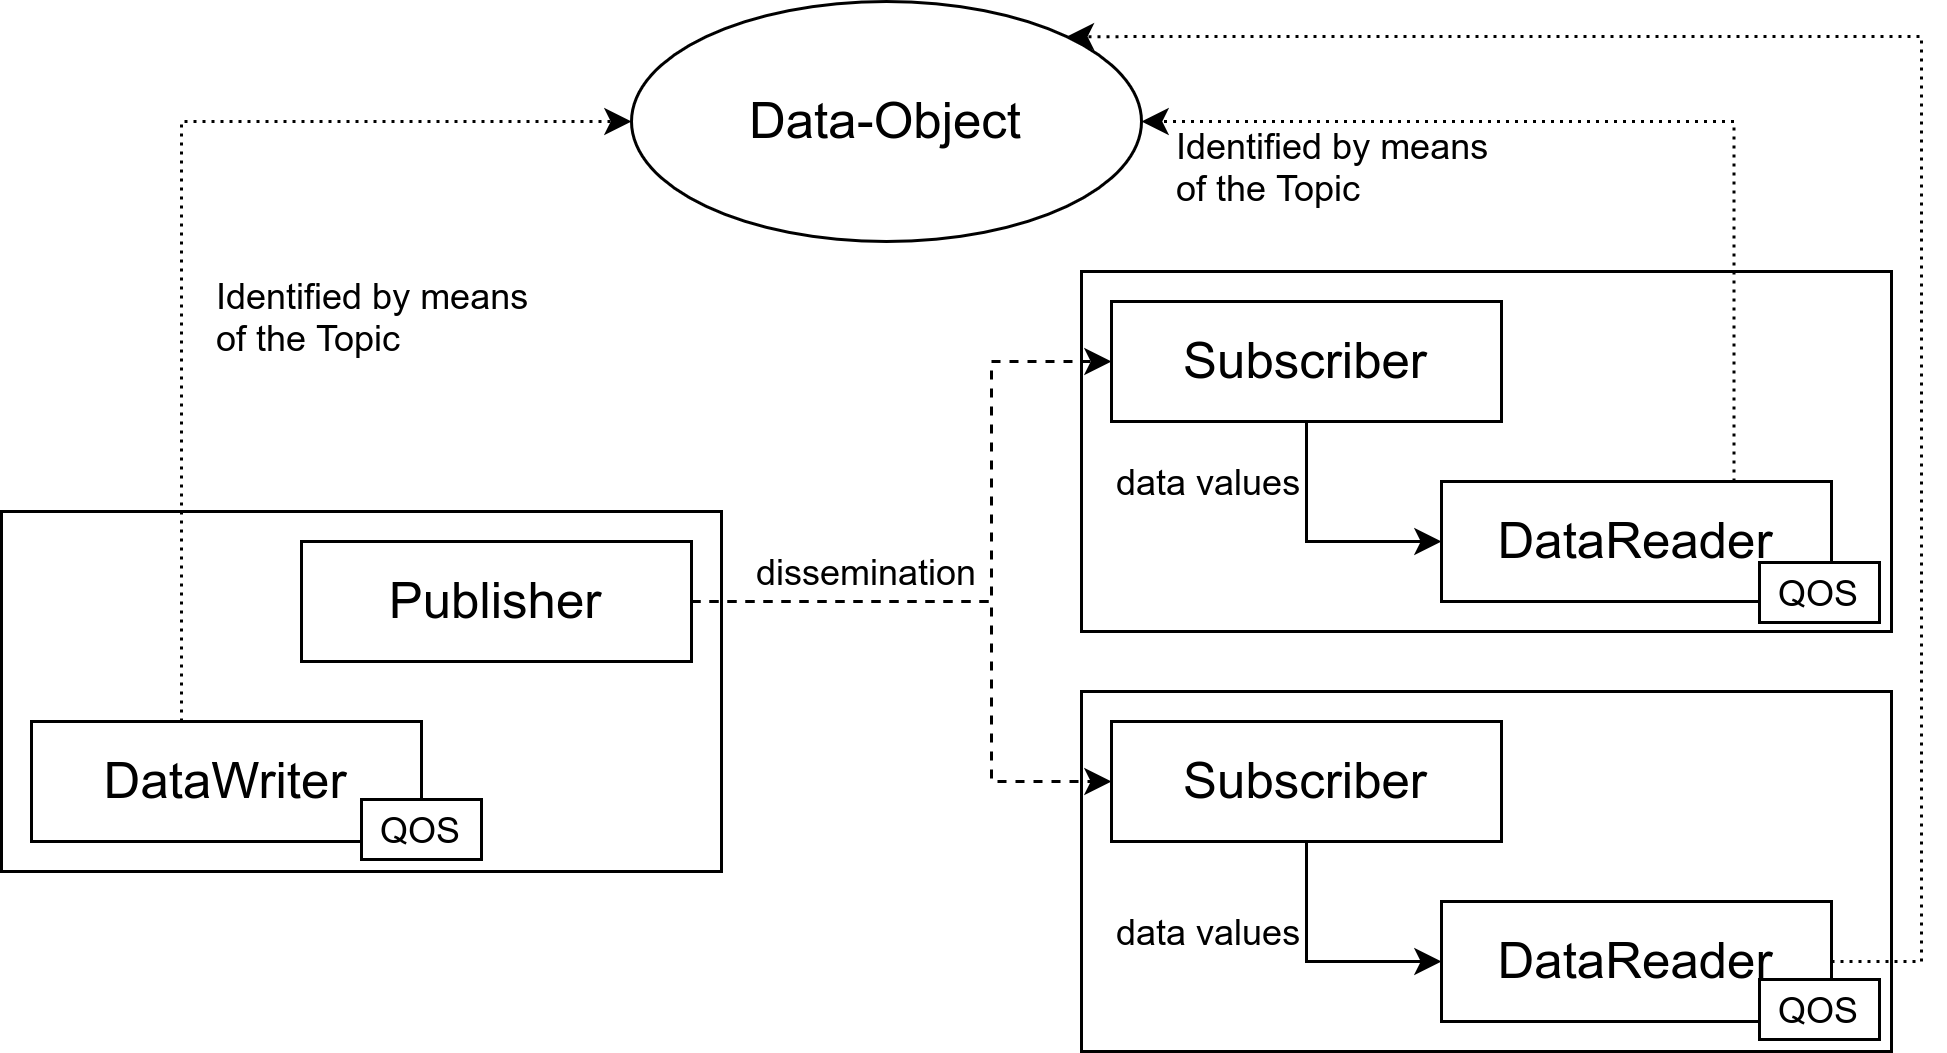
\includegraphics[width=0.75\linewidth]{images/DDSStructure}
	\caption{The \glsentryfull{DDS} is a data-centric communication model and follows the publish/subscribe pattern. The publishing and subscribing attendees do not communicate directly with each other, but make use of topics to read and write data objects.}
	\label{fig:DDSStructure}
\end{figure}

\Gls*{DDS} is a \gls*{DCPS} model for machine-to-machine communication, that is specified by the \gls*{OMG}~\cite{omgDDSspec}.
It is stated that the model should, for practical use, be implemented as a middleware, to directly interface with the underlaying \gls*{OS}.
The model follows the concept of a global data space to facilitate data exchange among entities based on type and content.
Central entities in the design are \texttt{Publishers} and \texttt{Subscribers}, while data exchange is based on \texttt{Topics}.
A \texttt{Publisher} is used for sending data of different types.
In order to send specifically typed data, a \texttt{DataWriter} object is used, which acts as a typed interface to a \texttt{Publisher}.
On the other side, a \texttt{Subscriber} is used to receive data and to make it accessible to the receiving application.
The equivalent of the \texttt{DataWriter} for the \texttt{Subscriber} is the \texttt{DataReader} object.
A \texttt{Topic} acts as the connecting element between publishing entities on the one side and subscribing entities on the other.
Any forecasting of when and how data is published to a \texttt{Topic} or received by a \texttt{Subscriber} is made possible through so called \glspl*{QOS} policies.
This concept is illustrated in~\autoref{fig:DDSStructure}, which is based on the official \gls*{DDS} specification~\cite{omgDDSspec} and shows the information flow from the publishing to the subscribing side.

An application can either rely on the middleware to asynchronously notify it about the presence of new data through so called \texttt{Listeners}, or actively wait for new data by utalizing \texttt{WaitSets}.
A \texttt{WaitSet} can be attached with different \texttt{Conditions}, for example \texttt{ReadConditions}, and allows the application to wait until either one or more of the attached conditions are satisfied, or until it times out.
Examples for conditions are \texttt{ReadCondition} and \texttt{QueryCondition}.
The \texttt{ReadCondition} object allows to designate specific data samples and is met when the specified type of data is present in a \texttt{DataReader}.
A \texttt{QueryCondition} is a specified \texttt{ReadCondition} that further provides capabilities of filtering the data that is read through a \texttt{DataReader}.
\\

The usefulness of \gls*{DDS} for containerization technologies in automotive architectures has been studied by Kugele \etal~\cite{KugeleDataCentricForAuto}.
Although their findings are based on containerization technologies and are therefore not resilient for this work, Kugele \etal showed that the applicability of \gls*{DDS} with regards to safety, certification and security depends on the actual implementation's characteristics.
Therefore, Vortex OpenSplice DDS is used thoughout this thesis, which is being developed and maintained by ADLINK.

The applicability of the \gls*{DDS}-standard and of Vortex OpenSplice \gls*{DDS} for safety-critical railway applications has been demonstrated by Schmidt and van't Hag~\cite{SchmidtMissionCriticalChallenges}.
Their findings show, that OpenSplice \gls*{DDS}'s \gls*{QOS} policies allow predictable time and locality characteristics for data distribution.
Further, their work provides an overview about Vortex OpenSplice's \gls*{QOS} policies and features to ensure reliability, availability, data-delivery, and resource usage.

\section{Techniques for Safety and Reliability Evaluation}
\label{sec:techniquesSafetyReliability}
In order to profoundly express and analyze redundancy techniques towards their safety, reliability and fault-tolerance, it needs to be defined what these characteristics mean.
\\

Reliability is, by IEEE 610.12-1990, defined as the ability of a system or component to perform its required function under stated conditions for a specified period of time~\cite{ieee610.12}.
A circumstance where a system deviates from its requirement is called a system failure.
A failure is preceded by a fault, which describes a static defect of a system~\cite{AmmannOffutt2016}.
When a fault becomes active, it manifests itself as an error, which marks an incorrect internal system state.
An failure occurs as soon as the error affects the system's environment.

\begin{definition}
A failure of a system or a system component is a state, where its actual behaviour deviates from the its specified behaviour.
\end{definition}

The definition of reliability used in this work is the following:

\begin{definition}
A system's reliability is a function of time that expresses the probability for the system to operate as specified at a time $t_1$, given that it was operating as specified at time $t | t \leq t_1$.
\end{definition}

In other words, reliability is a system's ability to not have any failure for a specific period of time.

A system's safety is associated with its reliability, since it consitutes an extension of reliability~\cite{AvizienisDependability2001}.
In general, safety defines the absence of catastrophic failures on a system's environment.
When the presence of non-catastropic failures can be reliably detected and a safe state can be taken in case of failures, safety can be treated as reliability concerning catastropic failures.
In other words, safety can be expressed as a system's probability to not experience any fault that would lead to a catastrophic failure in a specific time span.

Based on these definitions, it can be conducted that a system's safety and reliability can only be finally assessed when the system's environment, the reliability of the system's components and the operations performed by the system are known.
In addition, the system's architecture and structure need to be aquainted.
Finally, in order to specifically evaluate a system's safety, possible faults and their consequences need to be known.
In order to be able to evaluate and compare different architectural pattern towards their safety characteristics, independently of the subsequently conducted operations, the definition of \texttt{intrinsic safety}, made by~\cite{BoulangerStandards}, is used in this work.

\begin{definition}
A system is said to be intrinsically safe if one can be certain that any failure of one or more components of that system will only result in its becoming more permissive.
In the railway context, a complete stoppage is generally the safest state.
\label{def:intrinsic_safety}
\end{definition}

This definition requires that measures are taken to assure the system's safety even in the presence of failures.
A system that provides the functionality to behave as specified even in the case of faults is said to be fault tolerant~\cite{AvizienisDependability2001}.
Fault tolerance is generally obtained through error detection, which allows the system to determine the presence of errors and enables it to mitigate resulting failures.
In the course of this thesis, a system is considered to be safe when it is reliable and utalizes error detection mechanisms to ensure its intrinsic safety.
\begin{definition}
A system, in the course of this thesis, is said to be safe when it operates reliably and applies error detection mechanisms in order to be fault tolerant.
\label{def:safety}
\end{definition}

Thus, in order to be considered secure, a distributed system must tolerate possible faults that could occur in distributed systems.
Flaviu Cristian has established the following five fault classes for distributed distributed systems~\cite{CristianFaultModel}:

\begin{enumerate}
\item \textbf{F1:} One or multiple components in the system crash (\textbf{crash fault}).
\item \textbf{F2:} One or multiple components fail to respond to an incoming request (\textbf{omission fault}).
\item \textbf{F3:} One or multiple components fail to produce an output within a certain time span (\textbf{timing fault}).
\item \textbf{F4:} One or multiple components produce a wrong result (\textbf{computation fault}).
\item \textbf{F5:} One or multiple components produce arbitrary responses at arbitrary times (\textbf{byzantine fault}).
\end{enumerate}

It applies, that all fault classes \textbf{Fx} are included in \textbf{Fy}, given that $y \geq x$.
In the course of this thesis, the fault classes \textbf{F1} to \textbf{F4} are analyzed and byzantine faults are not covered.

\subsection{Safety Evaluation}
\label{sec:safetyEvaluation}
A required condition for a system to be safe is that the system is reliable (definition~\autoref{def:safety}).
One method of analyzing a system's reliability is through mathematical functions of time, for example the \texttt{exponential failure law}~\cite{GeffroyMotetDependableComputing}.
It describes a component's reliability as an exponential function on time.
\begin{equation}
R(t) = e^{-\lambda t}.
\label{eq:expFailureLaw}
\end{equation}
The parameter $\lambda$ is called the failure rate and encodes the probability of failures occuring in a certain time span, typically in an hour.
For the exponential failure law it is, mathematically, assumed that the components fail independently.
This might not always be the case in practice, as common core or power outage failures can affect multiple components at once.
However, the probability of failures affecting multiple components at once can be reduced by various techniques, such as using independent power supplies or diverse redundancy, the latter of which being discussed below.
\\

Among various theoretical techniques for evaluating a system's safety, Markov chains are one of the most commonly used~\cite{BarryFaultToleranceAnalysis}.
Markov chains are a stochastic process that models the alterations of a system's state and probabilities for the system to transition into a specific state given that it was in a certain state~\cite{KemenyMarkovChains}.
Thereby, the next state only depends on the current state and is independent from all previous system modifications.

For a safety analysis, each state models the system in one out of three conditions:
\begin{enumerate}
\item The system functions without having an error.
\item The system detects and successfully mitigates an error without leading to a failure
\item The system either not detects an error or does not recover from it, leading to a failure
\end{enumerate}

For the state transition probabilities, the exponential failure law~\autoref{eq:expFailureLaw}, with a constant failure rate $\lambda$, holds.

\begin{figure}[!hb]
	\centering
	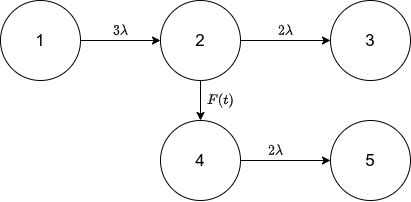
\includegraphics[width=0.75\linewidth]{images/TriplexSystemNASA}
	\caption{A reliability model for \glsentryfull{TMR} using Markov chains. In state (1), three replicas are operating redundantly. Each state transition describes the failure of a replica together with the corresponding probability.}
	\label{fig:NASATMR}
\end{figure}

An example Markov chain for a system using three replicas is proposed by NASA and depicted in~\autoref{fig:NASATMR}~\cite{NASAMarkovChains}.
At state (1), assuming that the system is homogeneous redundant, the probability that one of the replicas fails is $3\lambda$.
In state (2), the system applies failure detection and mitigation procedures and has a chance of $F(t)$ for successful reconfiguration, which allows the system to continue its work.
However, there is still a change of $2\lambda$ that another component fails before the system detects and mitigate the first failure, which would lead to a system fault and render the entire system unsafe.
In state (4), there is again a $2\lambda$ change for one of the remaining components to fail, which would lead to a failure of the entire system.

As experiments have shown, a system's recovery time is not necessarily exponential~\cite{TheoryAndPracticeReliableSystem}.
Thus, it is expressed by $F(t)$ which is the probability that the system recovers within a timespan less than $t$.

In a diverse redundant system, each component failure is represented with an individual state.

\section{Redundancy Patterns}
\label{sec:redundancyPatterns}
Redundancy is a typically applied technique for handling and masking errors in a system~\cite{TanenbaumSteen07}.
Error masking is the concept of detecting and mitigating errors, so that they do not become failures and effect the system's environment.
For redundancy, additional resources or information are added to a system, that would not be required when errors where impossible to happen in the system.
Barry Johnson defines redundancy in the following way~\cite{BarryFaultToleranceAnalysis}:
\begin{definition}
The concept of redundancy implies the addition of information, resources, or time beyound what is needed for normal system operation.
Redundancy can take one of several forms, including hardware, software, information, and time redundancy.
\end{definition}

Each form of redundancy has its unique characteristics and patterns, which are presented in the following.

\subsection{Hardware Redundancy}
In hardware redundancy, additional replications of physical components are added to the system.
This typically increases the system's safety by masking internal failures, but also increases the system's cost.
In general, a system's safety can be further improved when using components that are based on different internal components.
Using different components in redundancy patterns is called diverse redundancy, while replicating the same components is called homogeneous redundancy~\cite{HomogeneousRedundancyOuzineb}.
Using diverse redundancy has the benefit that it reduced the effect that common core errors have on a system's or component's safety.

Johnson subdevides hardware redundancy into two parts, namely passive and active redundancy.
In passive hardware redundancy, a voter or consensus algorithm is used to reduce a number of redundant outputs to a single output, in order to prevent individual internal failures from propergating out of the system.
In active hardware redundancy, the system tries to detect and repair any internal failure, for example by replacing the faulty component.
While \gls*{MOON} systems are a typical example of passive hardware redundancy, standby redundancy is often used as an example of active hardware redundancy.

A voter can be realized in software and in hardware.
The benefits of software voters are, that they typically cost less and are easier to develop, because no special hardware is required.
However, software voters operate slower and the approval process is more complicated, because additional hardware and software is used, that does not contribute to the voting.

The benefit of hardware voters is, that they can operate faster and a minimal set of hardware needs to be approved, which reduces the time and cost expenses for approving the system.

Both types of voters have in common, that they require some kind of time constraint synchronization with the replicas to collect their intermediate results, perform a voting, and recognize failed or delayed redundant results.
Therefore, the indivudual replicas communicate their results to the voter, which collects the results, performs the voting and thereby generates a single system result.
The voting process facilitates the system to allow single replicas to produce wrong results without rendering the overall system result wrong.
In an active hardware redundant system, where the individual components are independent and communicate via a shared communication medium, the synchronization process is further impeded by the impossibility of agreeing on values in asynchronous distributed systems with faulty components~\cite{FLPProblemConsensus}.
Consequentely, a way for synchonizing the communication is required, which can be achieved through time constraints in form of timeouts.
This can be, for example, achieved by starting a timer after a first replica sent its result, or by letting the voter request the result from each replica.
In addition, an expired timeout can indicate crashed replicas or network partitions.

\paragraph{M-out-of-N Systems}
\begin{figure}[!hb]
	\centering
	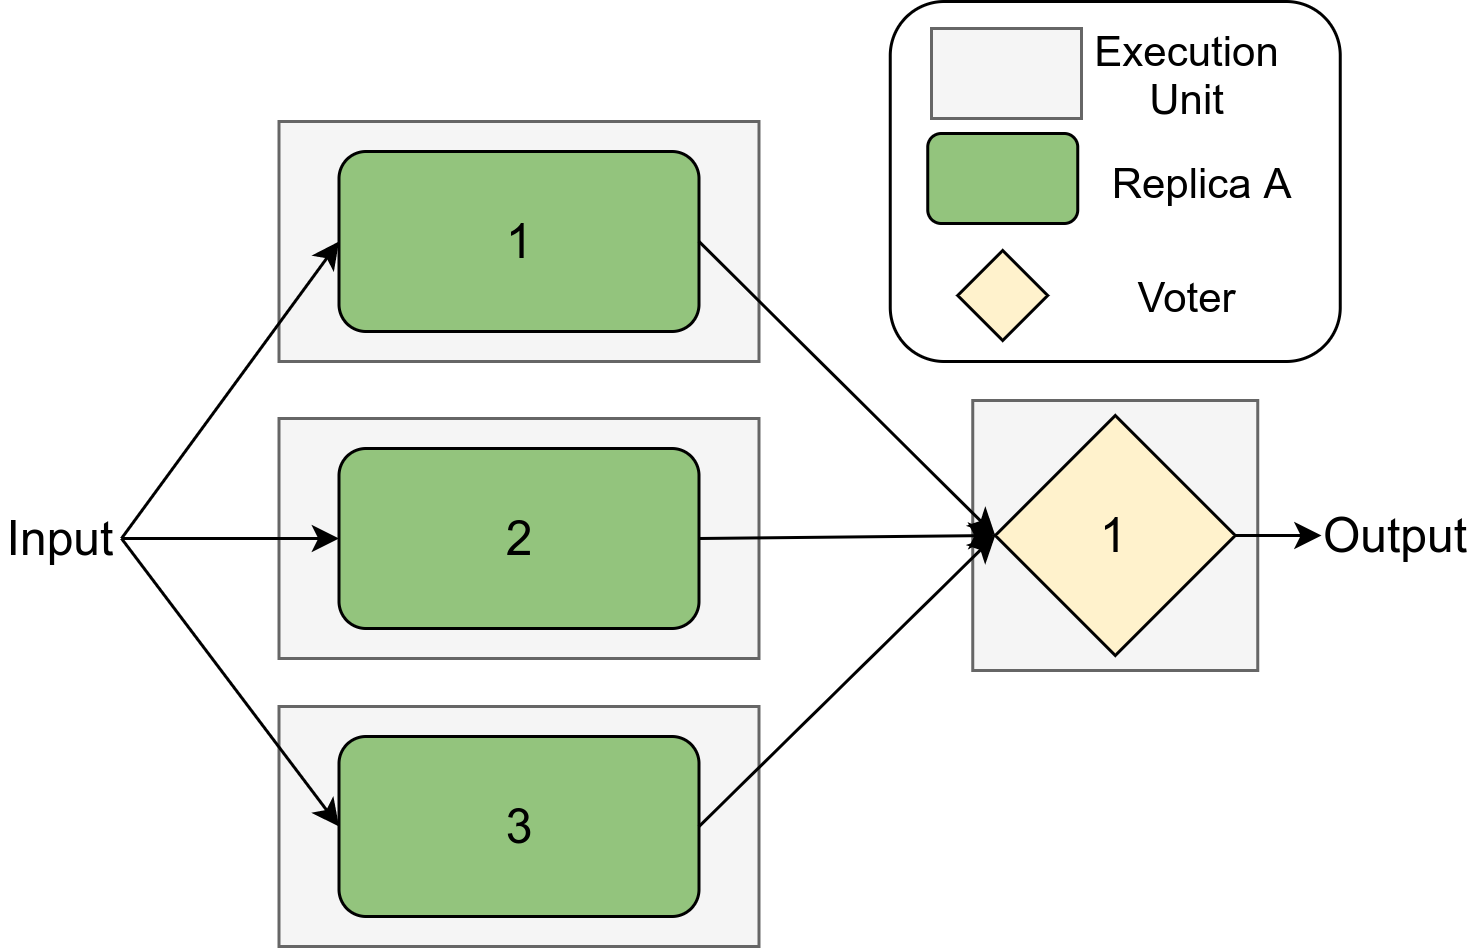
\includegraphics[width=0.75\linewidth]{images/Classical2OO3}
	\caption{Classical 3-out-of-2 redundancy, also known as \glsentryfull{TMR}. Three replicas are simultaneously reading and processing an input in a redundant way. A voter collects these redundant results and performs a majority voting to produce a final output.}
	\label{fig:Classical2OO3}
\end{figure}

One of the most common versions of \gls*{MOON} systems is \gls*{TMR}~\autoref{fig:Classical2OO3}.
In \gls*{TMR}, three replicas are receiving the same input and performing the same work in parallel.
A voter collects the individual outputs and reduces them to a single system output based on majority voting.
The system output must qualify the characteristic that at least two out of the three replicas agree on this output.
This allows the entire system to still produce a correct output even in the presents of a faulty replica.
All replicas, as well as the voter, are running on individual execution units.

Instead of having one voter that decides about the final result, the calculations could be modularized and votings on intermediate results could be made.
This would have the benefit of masking intermediate faults and not letting them influence further calculations.
An example of how this could be achieved is depicted in~\autoref{fig:IntermediateVoting}.
\\

The biggest weakness of \gls*{TMR} is the voter, because it marks a single point of failure.
Therefore, the voter's reliability in the system has to be high compared to the remaining replicas, because the entire system's reliability cannot be higher than the voter's reliability.
There is a lot of research for making voters more reliable, one of which being Arifeen \etal, who proposed a highly reliable hardware voter~\cite{ArifeenFaultTolerantTMR}.
An alternative to voters are consensus algorithm, where all components, not only a single voter, are involved in deciding about the system's output value~\cite{lamport2001paxos}.
While not having a single point of failure anymore, consensus approaches typically introduce a communication overhead and lead to rigid configurations~\cite{GamerIncreasingMOON}.

\begin{figure}[!hb]
	\centering
	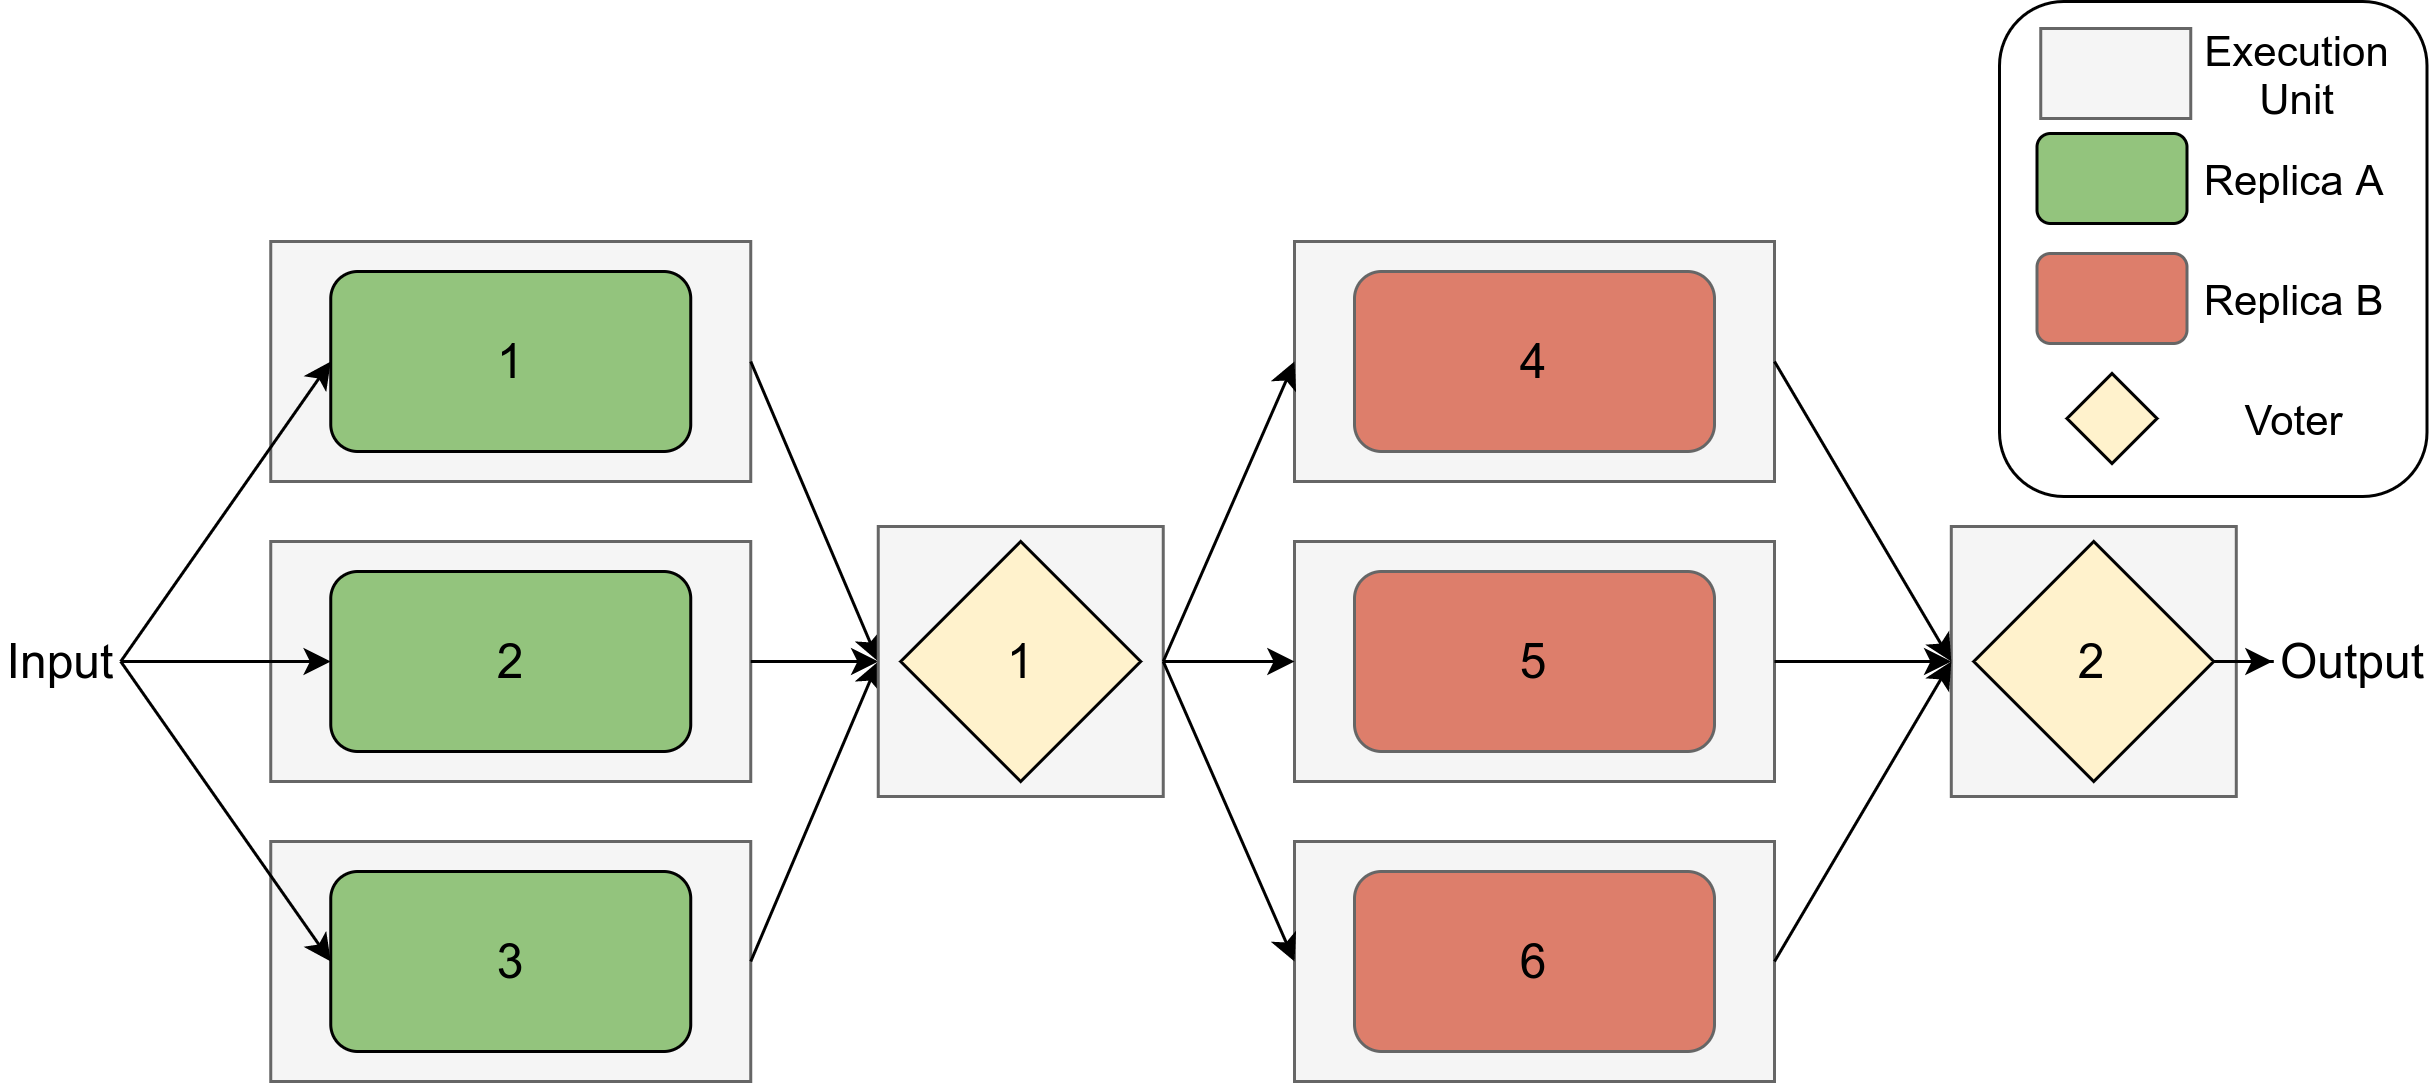
\includegraphics[width=0.75\linewidth]{images/IntermediateVoting}
	\caption{Intermediate voting could be applied to reduce the effect of partial results on the final output. Another benefit of this approach is its pipelined fashion, which improves the overall system throughput.}
	\label{fig:IntermediateVoting}
\end{figure}

\paragraph{Standby Redundancy}
\begin{figure}[!hb]
	\centering
	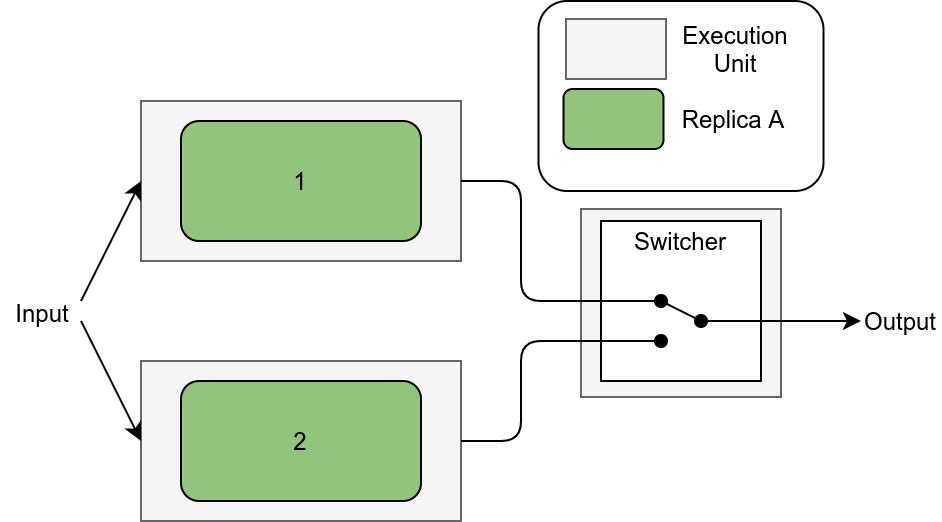
\includegraphics[width=0.75\linewidth]{images/ActiveSelectionRedundancy}
	\caption{With standby redundancy, a system can recover from individual component errors by replacing faulty components. Therefore, a switcher component performs error detection operations and delegates control over the output to the component it considers to be the most trustworthy.}
	\label{fig:StandbyRedundancy}
\end{figure}

As stated above, standby redundancy is an example of active hardware redundancy and builds on the concept of error detection, location and recovery.
When, in an exemplary case, an individual component experiences a fault, the resulting error needs to be detected and the faulty component needs to be located, so that the system can recover from the error by replacing the faulty component by an identical spare component.
This concept is depicted in~\autoref{fig:StandbyRedundancy}, where two identical replicas are used, one as a primary and one as a secondary component.
A switching element observes the active component and, when no error is detected, provides control about the system's output to the active components.
As soon as the switching element detects an error, it excludes the active component from the system and transfers control about the system's output to the secondary component, which thereby becomes the active component.
When the secondary component is already running when the switching happens, this is called hot standby redundancy.
When the secondary component needs to be turned on before it can be used as the active component, this is called cold standby redundancy.

\subsection{Software Redundancy}
One speaks of software redundancy, when the redundancy concepts or error detection methods are implemented in software.
Examples for software redundancy are heartbeat messages to validate a component's accessibility, component-checking, or software voters.
In component-checking, a a software or hardware program is used to monitor and validate a component's hardware, for example its memory, its clock, or its \gls*{CPU}.
\todo{principles of self-checking processor design}
A \abr{CPU}, for example, can apply redundant hardware for self-testing and fault-secureness~\cite{}.


Thereby, it can be qualified whether a specific component's output can be considered valid or not.
This state is summarized into the term \texttt{internal consistency}.

\begin{definition}
A system or a component is said to be internally consistent, when any failure of this component is not based on a fault of its internal hardware.
A system's or component's internal consitency can be determined by component checking mechanisms.
\end{definition}

By implication, when a system is internally consitent, any system failures can only be introduced by external causes, such as network delays, errors during data transmission, or defects in the inputs.

Further, voting or consensus algorithms can be implemented in software.
Similar to homogeneous and diverse hardware redundancy, diverse implementations of the same software can be used to reduce the effect of faults in a software.
The concept of diverse software programs is summarized under the term N-version programming, where a software program, which is based on the same specification, is developed by separate programmers~\cite{BarryFaultToleranceAnalysis}.

\subsection{Information and Time Redundancy}
The addition of redundant information can allow the detection, masking and recovery from faults~\cite{BarryFaultToleranceAnalysis}.
Examples for information redundancy include Hamming codes~\cite{HammingCodes}, checksums or information duplication.
In Hamming codes, multiple parity bits are attached to the data bits so that defects in the transmitted information can be detected.
Additionally, Hamming codes also allow to locate and correct errors in a bitstream.
All information redundancy concepts share that they somehow encode redundancy into the transmitted data that can later be decoded.

\begin{figure}[!hb]
	\centering
	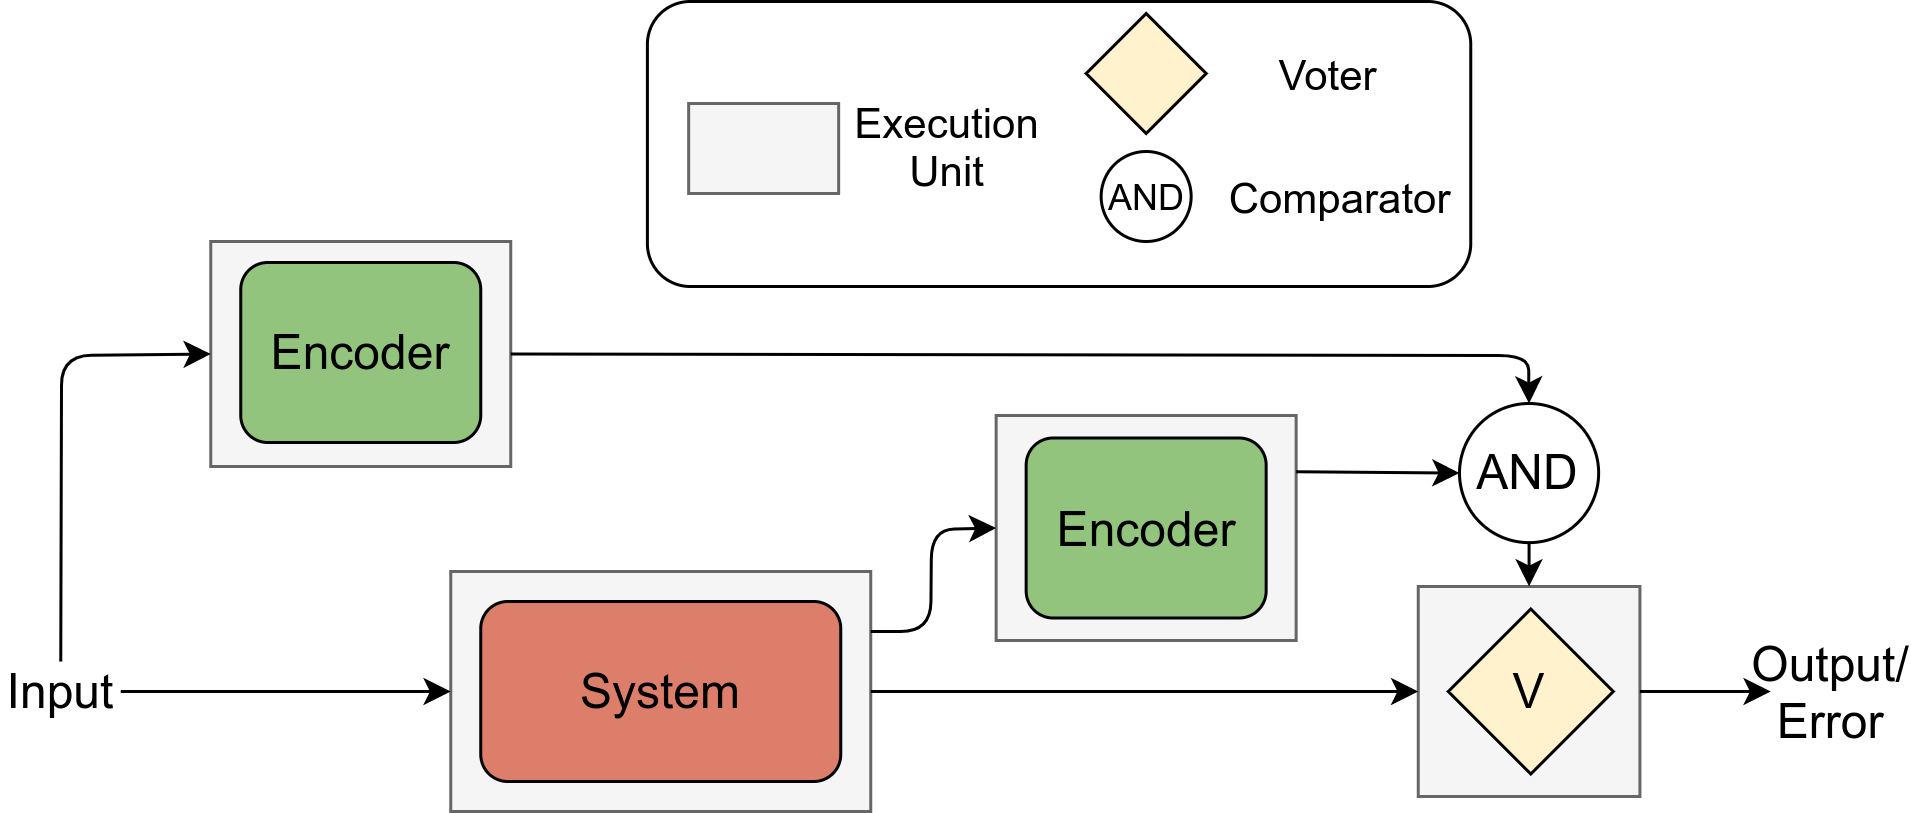
\includegraphics[width=0.75\linewidth]{images/ECC}
	\caption{\glsentryfull{ECC} applies both time and information redundancy. An encoder is used to encode both input and output of a system (time redundancy). This encoded information is used in addition to the actual data (information redundancy). The encoder function needs to be choosen to that possible outputs can be derived from it~\cite{Su2005ECC}. An exemplary encoding that fulfills these characteristics are Hamming codes~\cite{HammingCodes}.}
	\label{fig:ECC}
\end{figure}

Another way of adding redundancy is to perform the same operation multiple times at different points in time.
This concept is called \texttt{Time Redundancy} and has the benefit that it does not necessarily require additional physical components.
Thereby, permanent faults in a system can be detected.

\autoref{fig:ECC} depicts an example of a combination of information and time redundancy using \gls*{ECC} techniques.
Therefore, an encoder encodes the input and transmits this redundant information together with the input data.
After the system produces an output based on its input information, the output is also encoded and afterwards compared to the encoded input.
When there are anomalies between the system's input and its output, safety operations can be initiated.
The encoding function must be choosen so that it allows the detection of faults in the system, such as arithmetic shifting.

\section{Related Work}
\paragraph{Redundancy to enhance Safety.}
Alapan Chakroborty demonstrates a development process of a reliable, safe and fault-tolerant system using redundancy methods by an example of railway signalling~\cite{ChakrabortyFaultTolerantRailway}.
He argues, that every fault tolerant system needs to build upon real-time software solutions.
This requires both logical, as well as timing correctness, which can only be achieved by correct redundancy management such as fault propagation, synchronization and consensus among replicas.
At a fail-safe design's heart lies fault idenfication, masking and recovery.
Therefore, in a first step, each redundant design should be subdevided into redundant elements that are not affected by any fault from outside the element.
Chakroborty calls these redundant elements \glspl*{FCR}.
As a second step, he proposes to define interface between the \glspl*{FCR} so that they do not interfere with each other.
These two steps form a necessary precondition to be able to predict the probability of failures in the system.

In order for the system to reduce redundant results to a single result and to mask failures, the concept of voting is demanded.
Voting, as Chakraborty claims, requires the \glspl*{FCR} to be in identical states, to provide all redundant hardware with the same input and to ensure a real-time concurrent operation of the same computations on each \gls*{FCR} for synchronization.
Finally in the work, the shown method is performed on developing a railway signalling system.

An overview about possible redundancy concepts for the railway domain is provided by Bemment \etal~\cite{BemmentEvaluationOfRedundancy}.
They further made a cost, benefit and performance analysis for each presented concept.
\\

In my work, the concepts proposed by Bemment \etal are extended based on the steps by Chakraborty and by using and evaluating the feasibility of \gls*{DDS} for redundancy in the railway context.
Normally, as Bemment \etal pointed out, an in depth redundancy evaluation towards safety and reliability can only be made for well defined use cases where hazards, risks and potential accidents are know.
In my work, however, only the intrinsic safety in examined, which can be done theoretically without doing an exact risk analysis.
For further evaluations, an overview about about possible accidents in railway is given by~\cite{ERTMSRailwayAccidents}.
\\

\paragraph{Software development in the railway context.}
The CENELEC 50128 standard is a norm for software creating processes for railway applications, so that the build software can be considered safe.
The 2011 version of CENELEC 50128, as well as resources needed to achieve a set level of assurance, are presented by Jean-Louis Boulanger~\cite{BoulangerStandards}.
Conducting a CENELEC 50128 conform design process for all software artefacts created in this thesis is outside of its scope.
However, each software indended to be used in railway practice should pass the CENELEC 50128 norm.
\\

\begin{table}[h!]
	\begin{center}
		\caption{\glsentryfull{QOS} policies that affect the communication overhead (o) or the communication time (t). Each \abr{QOS} policy can either be applied to \texttt{DataWriters} (DR), \texttt{DataReaders} (DR), \texttt{Topics} (T), or \texttt{Publishers} (P).}
		\label{tab:qos_garciavalls}
		\begin{tabularx}{\textwidth}{|l|l|X|}
			\hline
			\textbf{QoS policy} & \textbf{Entity} & \textbf{Description}\\
			\hline \hline
			Deadline (t) & DR \& DW & Maximal expected elapsed time between arriving data samples or instances. Max committed time to publish samples or instances.\\
			\hline
			Reliability (o) & DR \& DW & Global policy that specifies whether or not data will be delivered reliably. It can be configured on a per DataWriter/-DataReader connection. \\
			\hline
			History (o) & DR \& DW & Stores sent or received data in cache. It affects the Reliability \gls*{QOS} policy. \\
			\hline
			Resource Limits (o) & DP & Limit to the allocated memory. It limits the queue size for History when the Reliability protocol is used. \\
			\hline
			Latency Budget (t) & T \& DR \& DW & Indication on how to handle data that requires low latency. Allow specification of maximum acceptable delay from time the data is written to the time the data is received by the subscriber. \\
			\hline
			Time based Filter (t) & DR & Limits the number of data samples sent for each instance per a given time period. \\
			\hline
			Transport Priority (t) & DW & Establishes a given priority for the data sent by a writer.\\
			\hline
		\end{tabularx}
	\end{center}
\end{table}

\paragraph{\abr{DDS} in safety-critical systems.}
The \gls*{DDS} is already successfully deployed in distributed time- and safety critical environments.
One example is given by Bijlsma \etal~\cite{DistributedSafety2020}, who extended the E-Gas layered monitoring concept to handle faults in a distributed and redundant system.
\Gls*{DDS} is applied to facilitate a reliable communication among individual components in the system.
An other example is given by Hadiwardoyo and Gao, who proposed the use of \gls*{DDS} in security cameras for subways using \glspl*{QOS}~\cite{DDSInSubways}.
Song \etal have proposed a system architecture that integrates the \abr{DDS} middleware into real-time embedded systems as well as safety-critical systems and thereby achieved a stable communication time~\cite{SongDDSInRealTimeSystems}.
Their approach has been varified by an \abr{UAV} combat scenario that operates in highly safety-critical scenarios.
Results have shown that the worst case communication time for a one kilkobyte payload and a relibale communication \abr{QOS} is around 280 microseconds.

Since Song \etal exerted a topology which is similar to the one used in this work - namely a network switch with a 100~Mpbs Ethernet link for communication and external nodes - their findings can be seen as a affirmation for the approach used in this work.
However, they utilized a different \abr{DDS} implementation, so that their experiments need to be repeated in my case to approve their findings. 
\\

A more general approach of how \gls*{DDS} can be used for enabling communication in distributed as well as time- and safety-critical environments, is given by García-Valls \etal~\cite{GarciaVallsDDSInDistributed}.
They used a design of reading and monitoring sensor data to benchmark the middleware's communication performance with different \glspl*{QOS}.
One of their findings is a summary of \gls*{QOS}-policies that effect the system's communication overhead and communication time.
These are illustrated in~\autoref{tab:qos_garciavalls} and are especially important when examining real-time and mission-critical systems.
The results from García-Valls \etal show that the communication performance remains stable even under heavy load.
Even though they applied a different \gls*{DDS} implementation than I did, the network topology and used hardware are comparable, which renders the results from García-Valls \etal useful for my work.

\paragraph{Time and availability for consensus based redundant systems.}
While redundant and distributed architectures are a typical approach to enhance a system's robustness, they also entail the demand to agree on certain data values, where the computations are based on.
Consensus algorithms are a way for components to coordinate and come to an agreement.
However, consensus algorithms also introduce a performance overhead, whose effects on the system's response time have been investigated by Sakic and Kellerer~\cite{SakicTimeInConsensus}.
Their studies focused on \abr{SDN} systems and \texttt{Raft}~\cite{RaftConsensusPaper}, a distributed consensus algorithm that takes care of data replication and leader election.
Results show that a system's response time in case of a random replica failing is linked to the probability of the leader being effected because this would entail a leader election process.
Eventually, in the studies from Sakic and Kellerer after one second, the cluster is almost guaranteed to deliver a response, even in the case of a random replica failing.
The situation looks different for combined correlated hardware and software failures, where only around 20\% of the systems respond a result after one seconds, when more than half of the replicas are affected.
In order to address this problem, Sakic and Kellerer propose a watchdog mechanism, which drastically increased the response probabilities in their experiments.

Based on the work from Sakic and Kellerer, the availability and response time for an actual system need to be evaluated in this work.
Further, the watchdog concepts should be kept in mind as it has a high impact on the system's response time in case of individual component failures.